\documentclass[12pt]{article}

\usepackage[dvips,letterpaper,margin=0.75in,bottom=0.5in]{geometry}
\usepackage{cite}
\usepackage{slashed}
\usepackage{graphicx}
\usepackage{amsmath}
\usepackage{amssymb}
\usepackage{braket}
\usepackage[american,fulldiode]{circuitikz}

\begin{document}
\newcommand{\ihbar}{\ensuremath{i \hbar}}
\newcommand{\dPsidt}{\ensuremath{ \frac{\partial \Psi}{\partial t} }}
\newcommand{\dPsidx}{\ensuremath{ \frac{\partial \Psi}{\partial x} }}
\newcommand{\ddPsidx}{\ensuremath{ \frac{\partial^2 \Psi}{\partial x^2} }}
\newcommand{\dPssdt}{\ensuremath{ \frac{\partial \Psi^*}{\partial t} }}
\newcommand{\dPssdx}{\ensuremath{ \frac{\partial \Psi^*}{\partial x} }}
\newcommand{\ddPssdx}{\ensuremath{ \frac{\partial^2 \Psi^*}{\partial x^2} }}

\newcommand{\dphidt}{\ensuremath{ \frac{d \phi}{dt} }}
\newcommand{\dpsidx}{\ensuremath{ \frac{d \psi}{dx} }}
\newcommand{\ddpsidx}{\ensuremath{ \frac{d^2 \psi}{dx^2} }}


\date{\vspace{-5ex}}

\title{Homework Assignment 4 \\ Relativistic Kinematics}

\maketitle

\noindent
All problems are graded on effort only. {\bf You may set $c=1$ whenever you like!}\\

\noindent
{\bf Griffiths: Problem 3.27}\\[3pt]

\noindent
{\bf Problem 1:}
Particle A of mass $M$ decays into particles B and C, each of mass
$m$, with $m < M/2$.  Particle A has momentum $p$, and the momentum of
particles B and C are at the same angle with respect to the momentum
of Particle A.  What is the magnitude of the momentum of particle B
($q$)?  What is the angle ($theta$) between the momentum of Particle A
and the momentum of Particle B?

\begin{center}
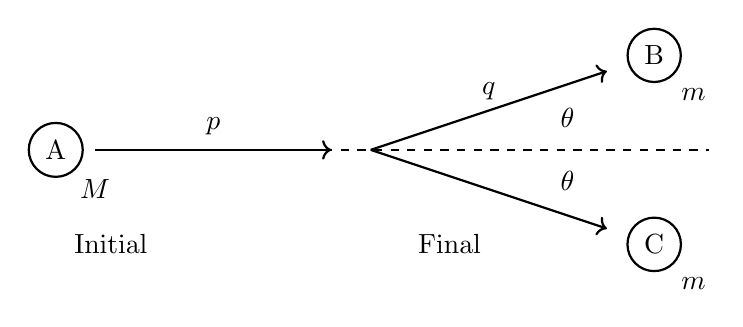
\begin{tikzpicture}[scale=1]
  \node[shape=circle,draw,thick] at (0,0) {A};
  \draw[->, thick] (0.5,0) -- ++(3.0,0);
  \draw[dashed, thick] (1.3,0) -- ++(7,0);
  \node at (0.5,-0.5) {$M$};
  \node at (2.0,0.3) {$p$};

  \node at (0.7,-1.2) {Initial};

  \draw[->, thick] (4,0) -- ++(3.0, 1.0);
  \draw[->, thick] (4,0) -- ++(3.0,-1.0);
  \node at (6.5,-0.4) {$\theta$};
  \node at (6.5, 0.4) {$\theta$};

  
  \node[shape=circle,draw,thick] at (7.6, 1.2) {B};
  \node at (8.1,0.7) {$m$};
  
  \node[shape=circle,draw,thick] at (7.6,-1.2) {C};
  \node at (8.1,-1.7) {$m$};
  
  \node at (5.5, 0.75) {$q$};
  
  \node at (5.0,-1.2) {Final};
\end{tikzpicture}
\end{center}


\noindent
{\bf Problem 2:}
Particles A and B each of mass $M$ collide to produce particles $1$
and $2$ each of mass $m$.  In the center of mass frame, particles A
and B have magnitude of momentum $p$.  What is the magnitude of the
momentum of particle 1 ($q$)?

\begin{center}
\begin{tikzpicture}[scale=1]
  \node[shape=circle,draw,thick] at (0,0) {A};
  \draw[->, thick] (0.5,0) -- ++(1.4,0);
  \node at (0.5,-0.5) {$M$};
  \node at (1.0,0.3) {$p$};

  \node[shape=circle,draw,thick] at (4,0) {B};
  \draw[->, thick] (3.5,0) -- ++(-1.4,0);
  \node at (4.5,-0.5) {$M$};
  \node at (3.0,0.3) {$p$};

  \node at (2.0,-1.2) {Initial};


  \node[shape=circle,draw,thick] at (6,-2) {2};
  \draw[<-, thick] (6.3,-1.7) -- (7.8,-0.2);
  \node at (6.5,-2.5) {$m$};


  \node[shape=circle,draw,thick] at (10,2) {1};
  \draw[<-, thick] (9.7,1.7) -- (8.2,0.2);
  \node at (10.5,1.5) {$m$};
  \node at (8.7,1.2) {$q$};
  
  \node at (9.0,-1.2) {Final};
\end{tikzpicture}
\end{center}

\newpage

\noindent
{\bf Problem 3:}
For the decay $a \to 1 + 2$ show that in the CMS the magnitude of the momentum of particle 1 is:
$$p^* = \frac{c}{2m_a}\sqrt{\left(m_a^2-(m_1 + m_2)^2\right)\left(m_a^2-(m_1 - m_2)^2\right)}$$
Hint:  When duing serious algebra, don't move around numbers like $m_1$.  Instead, do something like:
$$m_a \to a, \hspace{0.5cm} m_1 \to b, \hspace{0.5cm} m_2 \to c$$
Treat yourself right!\\[5pt]

\noindent
{\bf Problem 4:}
For two-body scattering $a + b \to 1 + 2$, show that the Lorentz invariant flux term:
$$F \equiv 4 E_a E_b (v_a + v_b)$$
is equivalent to:
$$F = 4 c^3 \sqrt{ (p_a \cdot p_b)^2 - m_a^2 m_b^2 c^4 } $$
Hint: Calculate $F^2$ and then calculate $(p_a \cdot p_b)^2$.\\[5pt]

\noindent
{\bf Problem 5:}
Show that in the lab frame where $b$ is at rest, the Lorentz invariant flux term is:
$$F = 4 c^4 m_b p_a$$\\[5pt]

\end{document}




